\documentclass[pdf, 10pt, unicode]{beamer}

\usepackage[T2A]{fontenc}
%\usepackage[cp1251]{inputenc}
\usepackage[utf8]{inputenc}
\usepackage[russian,english]{babel}
\usepackage{minted}
\usepackage{graphicx}
\usepackage{amssymb}
\usepackage{amsthm}
\usepackage{amsmath}
\usepackage{tabularx}
\usepackage{multicol}
\usepackage{multirow}
\usepackage{calrsfs}
\usepackage{listings}
\usepackage{color}
\usepackage{hyperref}

\hypersetup{
  colorlinks, linkcolor=blue
}

\usepackage{array}
\newcolumntype{L}[1]{>{\raggedright\let\newline\\\arraybackslash\hspace{0pt}}m{#1}}
\newcolumntype{C}[1]{>{\centering\let\newline\\\arraybackslash\hspace{0pt}}m{#1}}
\newcolumntype{R}[1]{>{\raggedleft\let\newline\\\arraybackslash\hspace{0pt}}m{#1}}

% \lstset{basicstyle=\fontsize{7pt}{1em}\ttfamily,
%         keywordstyle=\fontsize{7pt}{1em}\color{MOOCBlue}\bfseries,
%         commentstyle=\fontsize{7pt}{:q1em}\ttfamily\color{MOOCGreen}}


\usepackage{caption}
\usepackage{subcaption}

% \lstset{language=C++,
%   basicstyle=\footnotesize\itshape,
%   keywordstyle=\color{black}\bfseries\underbar,
%   % underlined bold black keywords
%   identifierstyle={\color{black}},%
%   commentstyle=\color{brown}, % brown comments
%   stringstyle=\color{blue}\ttfamily, % typewriter type for strings, blue
%   showstringspaces=false
% }

\definecolor{MOOCGrey}{RGB}{230,230,230}
\definecolor{MOOCBlue}{RGB}{38,57,200}
\definecolor{MOOCGreen}{RGB}{38,130,63}

\lstset{extendedchars=true}
\lstset{language=C++, basicstyle=\small\ttfamily,  keywordstyle=\small\color{MOOCBlue}\bfseries,
        commentstyle=\small\ttfamily\color{MOOCGreen}, showstringspaces=false,
        extendedchars=true, texcl=true, frame=single,
        morekeywords={size_t}}



\newenvironment{changemargin}[2]{%
\begin{list}{}{%
\setlength{\topsep}{0pt}%
\setlength{\leftmargin}{#1}%
\setlength{\rightmargin}{#2}%
\setlength{\listparindent}{\parindent}%
\setlength{\itemindent}{\parindent}%
\setlength{\parsep}{\parskip}%
}%
\item[]}{\end{list}}


\usetheme{Copenhagen}
\usepackage{color}

\usecolortheme[RGB={50,100,200}]{structure}

\setbeamertemplate{navigation symbols}{}
\setbeamertemplate{itemize
item}{\scriptsize\raise1.25pt\hbox{\donotcoloroutermaths$\blacktriangleright$}}

\setbeamertemplate{frametitle continuation}[from second]

\title{Практика 1. Воспоминания про Linux. Воспоминания про получение двоичного кода (компиляция, ассемблер, линковка).}
\author{Евгений Линский}
\date{}
\usefonttheme[onlymath]{serif}

\setbeamerfont{institute}{size=\normalsize}

\setbeamertemplate{footline} {
  \hbox{%
  \begin{beamercolorbox}[wd=0.08\paperwidth,ht=2.5ex,dp=0ex,left]{title in head/foot}%
  \end{beamercolorbox}%
  \begin{beamercolorbox}[wd=0.46\paperwidth,ht=2.5ex,dp=1ex,center]{title in head/foot}%
    \usebeamerfont{title in head/foot}{C++}%\insertshortauthor %\insertshorttitle
  \end{beamercolorbox}%
  \begin{beamercolorbox}[wd=0.46\paperwidth,ht=2.5ex,dp=1ex,right]{date in head/foot}%
    \usebeamerfont{date in head/foot}
    \insertframenumber{} / \inserttotalframenumber{}\hspace*{2ex}
  \end{beamercolorbox}}%
  \vskip0pt%
}

\sloppy

\begin{document}
\begin{frame}
  \vspace{1cm}
  \large
  \maketitle
  \thispagestyle{empty}
  \vspace{1cm}
  \date{}
\end{frame}


\begin{frame}[fragile]{{\tt Воспоминания про Linux.}}

\begin{center}
  \huge{Воспоминания про Linux}
\end{center}

\end{frame}

\begin{frame}[fragile]{{\tt Что и как установить?}}

  \begin{itemize}
      \item Что?  \href{https://ubuntu.com/download/desktop}{Ubuntu} (самая распространенная)
      \item Как?
        \begin{itemize}
            \item второй ОС (установка сложнее, быстро работает)
            \item в \href{https://ldvsoft.net/2017/09/10/ubuntu-course.html}{виртуальной машине}
        \end{itemize}
      \item Что почитать? \href{https://drive.google.com/file/d/14ZxbYY8FWMdCDnHH1NhKj98cBA7ZiODJ/view?usp=sharing}{Основы Linux от основателя Gentoo}
  \end{itemize}
\end{frame}


\begin{frame}[fragile]{{\tt Что это?}}
\begin{tiny}
\begin{verbatim}
/
bin -> usr/bin
boot
cdrom
dev
etc
home
lib -> usr/lib
lib32 -> usr/lib32
lib64 -> usr/lib64
libx32 -> usr/libx32
lost+found
media
mnt
opt
proc
root
run
sbin -> usr/sbin
snap
srv
swapfile
sys
tmp
usr
var
\end{verbatim}
\end{tiny}
\end{frame}

\begin{frame}[fragile]{{\tt FHS}}
\begin{verbatim}
/ (корневая директория)
•/boot (статичные файлы загрузчика)
•/dev (файлы устройств)
•/etc (специфические для хоста конфигурационные файлы)
•/home (домашняя директория пользователя)
•/lib (основные разделяемые библиотеки и модули ядра)
•/mnt (точка монтирования для временных нужд)
•/opt (дополнительные пакеты ПО)
•/sbin (основные системные программы)
•/tmp (временные файлы)
•/usr (вторичная иерархия)
•/var (изменяемые данные)
\end{verbatim}
\end{frame}

\begin{frame}[fragile]{{\tt Командная строка }}
\begin{itemize}
  \item gnome-terminal (программа для ввода и вывода команд)
  \item bash (программа для выполнения команд)
  \item команды для работы с файловой системой
    \begin{itemize}
        \item cd dir (перейти в директорию), ls dir (посмотреть содержание директории)
        \item cp src dst (скопировать файл), mv src dst (переместить файл), rm dir (удалить файл)
        \item mkdir dir (создать директорию)
    \end{itemize}
\end{itemize}
bash: tab (автодополнение), arrows (предыдущая команда), Ctrl+R (поиск по истории)
\end{frame}

\begin{frame}[fragile]{{\tt Пути }}
\begin{itemize}
  \item Пусть в домашней директории пользователя elinsky есть директории caos и soac.
  \item В директории caos есть файл hello.S
  \item Мы находимся в директории soac.
  \item Как можно указать путь до файла hello.S
\end{itemize}

\begin{itemize}
  \uncover<2->{\item ls /home/elinsky/caos/hello.S}
  \uncover<3->{\item ls ../caos/hello.S}
  \uncover<4->{\item ls \textasciitilde/caos/hello.S}
\end{itemize}

\end{frame}

\begin{frame}[fragile]{{\tt Примеры }}

\begin{verbatim}
cd ~
mkdir caos
mkdir soac
cd caos
nano hello.S
cat hello.S
cp hello.S ../caos
rm hello.S
man rm
\end{verbatim}

\begin{itemize}
  \item nano -- консольный текстовый редактор (графический gedit)
  \item cat -- утилита для просмотра содержимого файла
  \item man -- документация по утилите rm
\end{itemize}

\end{frame}

\begin{frame}[fragile]{{\tt Примеры. Ключи командой строки. }}
\begin{verbatim}
cd ~
mkdir -p ~/a/c/d
ls -al
mkdir -p ~/x
cp -r ~/a ~/x
rm -rf ~/x
ls -al
\end{verbatim}
\end{frame}

\begin{frame}[fragile]{{\tt Как установить программу? }}
Собрать самому (make, зависимости)/установить пакет (репозитории).
\begin{verbatim}
sudo apt update
sudo apt search gcc
sudo apt install build-essential gcc-multilib
\end{verbatim}
\end{frame}

\begin{frame}[fragile]{{\tt gcc }}
  \begin{itemize}
    \item gcc -- набор компиляторов
    \item binutils -- линкер, ассемблер, дизассемблер
    \item gdb -- отладчик
  \end{itemize}
\end{frame}

\begin{frame}[fragile]{{\tt К следующей паре }}
  Хорошо бы:
  \begin{itemize}
    \item поставить Ubuntu (можно в виртуалке)
    \item поставить build-essential (gcc и все-все-все)
  \end{itemize}
\end{frame}

\begin{frame}[fragile]{{\tt Воспоминания про двоичный код.}}

\begin{center}
  \huge{Воспоминания про двоичный код}
\end{center}

\end{frame}


\begin{frame}[fragile]{{\tt Все хранится в числах}}

\begin{itemize}
  \item Компьютер умеет работать только с числами
    \begin{itemize}
        \item Текст. Кодировка задает соответствие между изображением символа и числовым кодом  ('A'  -- 65).
        \item Изображение. Цвет точки на экране --- три числа Red Green Blue  (черный --- 0 0 0).
        \item Команды, из которых состоит программа, тоже хранится в виде чисел.
    \end{itemize}
  \item Числа хранятся в двоичной системе счисления
    \begin{itemize}
        \item ``Есть сигнал/нет сигнала'' (1/0) [ложь! ложь! ложь!]
        \item ``Есть намагниченность/нет намагниченности'' (1/0)
    \end{itemize}
\end{itemize}

\end{frame}

\begin{frame}[fragile]{{\tt Схема компьютера}}

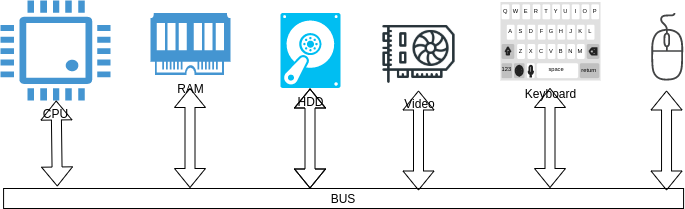
\includegraphics[scale=0.4]{scheme.png}

Можно сказать, что все что умеет процессор, это выполнять над числами арифметические и логические операции и пересылать
данные между периферийными устройствами:
\begin{itemize}
  \item арифметическая операция: загрузить числа из памяти в процессор, выполнить операции, выгрузить в память
  \item вывести пиксель: переслать координаты и цвет точки (RGB) в видеокарту
  \item сохранить файл: послать данные и их положение на диске в контроллер жесткого диска
\end{itemize}
\end{frame}

\begin{frame}[fragile]{{\tt Программирование в двоичных кодах}}

\begin{itemize}
  \item Архитектура процессора (x86, ARM, RISC-V): набор команд и регистры
    \begin{itemize}
        \item Регистры --- ячейки памяти внутри процессора (x86: размер -- 64 бита, количество -- 20)
    \end{itemize}
  \item Программа
  \begin{tabular}{ll}
    загрузить из ячейки RAM 300 в регистр1 & 1 300 1 \\
    загрузить из ячейки RAM 500 в регистр2 & 1 500 2 \\
    сложить регистр1 и регистр2 в регистр3 & 3 1 2 3\\
    выгрузить регистр3 в ячейку RAM 100 & 2 3 100 \\
  \end{tabular}
  \item 1 -- код команды загрузить, 2 -- код команды выгрузить, 3 -- ... сложить
\end{itemize}

\end{frame}

\begin{frame}[fragile]{{\tt Проблемы при программировании в кодах}}

\begin{itemize}
  \item Надо помнить о ячейках памяти и регистрах (какие заняты, какие нет)
  \item Коды команд плохо запоминаются
  \item Отсутствует переносимость: в разных архитектурах -- разные наборы команды, коды команд, наборы регистров
\end{itemize}

\end{frame}

\begin{frame}[fragile]{{\tt Ассемблер}}

\begin{itemize}
  \item Ассемблер -- транслятор (программа) из текста на языке ассемблер в двоичные коды.
  \item У команд и ячеек памяти есть символьные имена, которые легко запомнить.
  \item Программа:
 \begin{tabular}{ll}
    загрузить из ячейки RAM 300 в регистр1 & load data1, r1 \\
    загрузить из ячейки RAM 500 в регистр2 & load data2, r2 \\
    сложить регистр1 и регистр2 в регистр3 & add r1,  r2,  r3\\
    выгрузить регистр3 в ячейку RAM 100 & store r3, data3 \\
    & .data data1 300 data2 500\\
    & .data data3 100\\
  \end{tabular}
\end{itemize}

Какие проблемы остались? \uncover<2->{Переносимость!}

\end{frame}

\begin{frame}[fragile]{{\tt Язык Высокого Уровня (ЯВУ)}}
\begin{minted}[linenos=true]{cpp}
int a = 3;
int b = 5;
int c = a + b;
\end{minted}
\begin{itemize}
  \item Компилятор -- транслятор (программа) из текста на ЯВУ переводит в текст на языке ассемблера.
  \item Подбирает команды, ячейки памяти и номера регистров так, чтобы программа быстро выполнялась и занимала
  минимум памяти (за несколько проходов по тексту).
\end{itemize}
Программа --> [Компилятор] --> [Ассемблер] --> Исполняемый файл
\end{frame}

\begin{frame}[fragile]{{\tt Язык C}}

\begin{itemize}
    \item Bell Labs. Задача: создать переносимую ОС (должна работать на разных архитектурах).
    \item Язык для ОС Unix.  Язык C (``Write once, compile everywhere!''). Деннис Ритчи. 197X.
    \item Если для новой архитектуры существует (в современном мире --- обычно да) компилятор языка C,
    то программу не надо переписывать, а надо просто перекомпилировать этим компилятором.
\end{itemize}
    \uncover<2->{На самом деле нет: в стандартную библиотеку языка C не входит графика, сеть и т.д.}

\end{frame}

\begin{frame}[fragile]{{\tt Файлы}}
\begin{minted}[linenos=true]{cpp}
//main.c
int main() {
  int a = 3; int b = 5;
  int c = a + b;
  int d = sum(c, b);
  return 0;
}
\end{minted}
\begin{minted}[linenos=true]{cpp}
//util.c
int sum(int a, int b) {
  return a + b;
}
\end{minted}

\end{frame}

\begin{frame}[fragile]{{\tt Построение программы (build)}}

\begin{itemize}
  \item Скомпилировать (компилятор + ассемблер) main.c --> main.o (объектный файл)
  \item Скомпилировать util.c --> util.o
  \item Слинковать [Линкер] main.o, util.o --> main.elf
\end{itemize}

\end{frame}

\begin{frame}[fragile]{{\tt Линкер}}

main.o
\begin{verbatim}
1 300 1
1 500 2
3 1 2 3
2 3 100
call sum
...
\end{verbatim}

sum.o
\begin{verbatim}
func sum
43 500 2
4 1 2 3
4 3 100
...
\end{verbatim}

В объектном файле -- имена функций не заменены на адреса.

\end{frame}

\begin{frame}[fragile]{{\tt Линкер}}

main.elf
\begin{verbatim}
[20] 1 300 1
[24] 1 500 2
[28] 3 1 2 3
[32] 2 3 100
[36] 13  50
...
[50] 43 500 2
[54] 4 1 2 3
[58] 4 3 100
...
\end{verbatim}

Линкер (линковщик, компоновщик) должен склеить файлы вместе и заменить вызовы функции по имени на вызовы по адресу (процессор
понимает только числа -- адреса).

\end{frame}

\begin{frame}[fragile]{{\tt Библиотеки.}}

\begin{enumerate}
  \item Статические (*.a, *.lib): объектные файла из библиотеки присоеднияются к программе в момент линковки
    \begin{itemize}
        \item Легко установить (не нужно отдельно загружать библиотеку)
        \item При выходе новой версии библиотеки (например, исправлен баг) автору программы нужно послать пользователю пересобранную версию
    \end{itemize}
  \item Динамические (*.so, *.dll): хранятся отдельно, связывание программы и библиотеки происходит в момент выполнения (помогает отдельная компонента --- загрузчик )
    \begin{itemize}
        \item Необходимо отдельно установить все необходимые библиотеки (решение: packages and repositories)
        \item При выходе новой версии библиотеки (например, исправлен баг) пользователь может самостоятельно обновить только библиотеку без пересборки программы.
    \end{itemize}

\end{enumerate}

\end{frame}


\begin{frame}[fragile]{{\tt gcc }}
\begin{verbatim}
// собрать полностью с отладочными символамм
gcc -g hello.c -o hello.elf
// только компиляция и ассемблирование (без линковки)
gcc -c hello.c -o hello.o
// только компиляция
gcc -S hello.c -o hello.S
// только препроцессор
gcc -E hello.c -o hello.tmp
// дизассемблирование
objdump -D hello.elf >hello.bin
\end{verbatim}
\end{frame}

\begin{frame}[fragile]{{\tt Запуск и отладка }}
\begin{verbatim}
./hello.elf
echo $? // результат return из main
gdb hello.elf
\end{verbatim}
PATH -- путь для поиска исполняемых файлов (echo \$PATH)
\end{frame}

\begin{frame}[fragile]{{\tt GDB }}
\begin{verbatim}
layout src
break main
run
s
p/d varibale
layout asm
si
continue
quit
\end{verbatim}
Ctrl + x + o
\end{frame}

\begin{frame}[fragile]{{\tt Makefile }}

оступы -- tab!
\begin{verbatim}
hello.elf: hello.c
  gcc hello.c -o hello.elf

clean:
  rm -rf hello.elf

build: hello.elf
\end{verbatim}
\$> make

\end{frame}

\begin{frame}[fragile]{{\tt К следующей паре }}
  Хорошо бы:
  \begin{itemize}
    \item позапускать gcc в разных режимах
    \item позапускать gdb в разных режимах
  \end{itemize}
\end{frame}

\end{document}

